\documentclass[a4paper,12pt]{article}

%%% Работа с русским языком
\usepackage{cmap}					% поиск в PDF
\usepackage{mathtext} 				% русские буквы в фомулах
\usepackage[T2A]{fontenc}			% кодировка
\usepackage[utf8]{inputenc}			% кодировка исходного текста
\usepackage[english,russian]{babel}	% локализация и переносы
\usepackage{float}
%%% Дополнительная работа с математикой
\usepackage{amsfonts,amssymb,amsthm,mathtools} % AMS
\usepackage{amsmath}
\usepackage{icomma} % "Умная" запятая: $0,2$ --- число, $0, 2$ --- перечисление
\usepackage{setspace}
%% Номера формул
%\mathtoolsset{showonlyrefs=true} % Показывать номера только у тех формул, на которые есть \eqref{} в тексте.

%% Шрифты
\usepackage{euscript}	 % Шрифт Евклид
\usepackage{mathrsfs} % Красивый матшрифт

%% Свои команды
\DeclareMathOperator{\sgn}{\mathop{sgn}}

%% Перенос знаков в формулах (по Львовскому)
\newcommand*{\hm}[1]{#1\nobreak\discretionary{}
	{\hbox{$\mathsurround=0pt #1$}}{}}

%%% Работа с картинками
\usepackage{graphicx}  % Для вставки рисунков
\graphicspath{{images/}{images2/}}  % папки с картинками
\setlength\fboxsep{3pt} % Отступ рамки \fbox{} от рисунка
\setlength\fboxrule{1pt} % Толщина линий рамки \fbox{}
\usepackage{wrapfig} % Обтекание рисунков и таблиц текстом

%%% Работа с таблицами
\usepackage{array,tabularx,tabulary,booktabs} % Дополнительная работа с таблицами
\usepackage{longtable}  % Длинные таблицы
\usepackage{multirow} % Слияние строк в таблице
\usepackage[unicode, pdftex]{hyperref}
\usepackage{xcolor}
%\definecolor{urlcolor}{HTML}{0000ff}
%\definecolor{linkcolor}{HTML}{799B03}
%\hypersetup{pdfstartview=FitH,  linkcolor=linkcolor,urlcolor=urlcolor, colorlinks=true}
\setcounter{secnumdepth}{0}
\usepackage{csquotes}
\linespread{2} 
%%% Заголовок
\title{RL}
\author{Dimtirov Vladimir}
\date{\today}


\begin{document}
	\maketitle
	\newpage
	\tableofcontents
	\newpage
	\section{Markov decision process}
	
	MDP is tuple $\langle\mathcal{S}, \mathcal{A}, \mathcal{P}, \mathcal{R}\rangle$, where:
	
	\begin{itemize}
		\item $\mathcal{S}$ - set of states of the world
		\item $\mathcal{A}$ - set of actions
		\item $\mathcal{P}: \mathcal{S} \times \mathcal{A} \mapsto \triangle(\mathcal{S})$ - state-transition function, giving us $p\left(s_{t+1} \mid s_t, a_t\right)$
		\item $\mathcal{R}: \mathcal{S} \times \mathcal{A} \mapsto \mathbb{R}$ - reward function, given us $\mathbb{E}_R\left[R\left(s_t, a_t\right) \mid s_t, a_t\right]$
	\end{itemize}
	
	Reward hypothesis (R.Sutton) 
	\begin{displayquote}
		That all of what we mean by goals and purposes can be well thought of as maximization of the expected value of the cumulative sum of a received scalar signal (reward)
	\end{displayquote}
	
	Cumulative rewards is called a return: 
	
	$G_t \triangleq R_t+R_{t+1}+R_{t+2}+\ldots+R_T$
	
	
	There are \textbf{2 problems} in the design of the system:
	\begin{enumerate}
		\item Infinite sum -> solve: discounting coeeficient 
		\item Simple solve -> watch the pic \ref{fig:screenshot001}
	\end{enumerate}
	
	\begin{figure}[H]
		\centering
		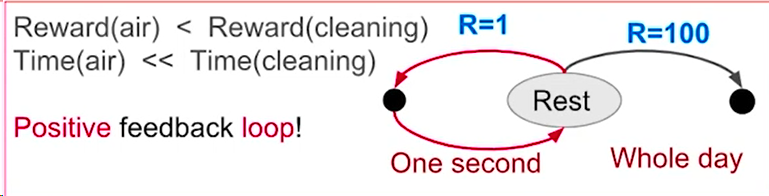
\includegraphics[width=1\linewidth]{../Image/screenshot001}
		\caption{Simple solution}
		\label{fig:screenshot001}
	\end{figure}
	

	Solving the infinite sum problem: get discounting coefficient ($0 \leq \gamma<1$) and cumulative rewards will take the form:
	
	
	$$\sum_{k=0}^{\infty} \gamma^k R_{t+k+1}$$
	
	This method has its pluses:
	
	\begin{itemize}
		\item Human likeness
		\item Mathematical convenience 
		\item fast optimization 
	\end{itemize}
	
	\textbf{Notes}: multiplying by $\gamma$ changes the task and it's solution!
	 
	
	\textbf{Take away 1:} reward only for what, but never for how
	
	\textbf{Take away 2:} do not subtract mean from rewards
	
	
	Transformation politic for reward (ML advice):
	
	\begin{itemize}
		\item Rewards scaling - division by positive constant
		\item Reward shaping - we could add to all rewards in MDP values of potential-based shaping function 
	\end{itemize}   

	\subsection{Expected objective}
	
	Optimal policy maximizes expected return: 
	
	$$\begin{aligned} \mathbb{E}\left[G_0\right] & =\mathbb{E}\left[R_0+\gamma R_1+\ldots+\gamma^T R_T\right] \\ & =\mathbb{E}_{E, \pi_\theta}\left[G_0\right] \\ & =\mathbb{E}_{\pi_\theta}\left[G_0\right] \\ & =\mathbb{E}\left[G_0 \mid \pi_\theta\right] \\ & =\mathbb{E}_{s_{0: T}}\left[G_0\right] \\ & =\mathbb{E}_{a_0: T}\left[\mathbb{E}_{a_0 \mid s_0}\left[R_0+\mathbb{E}_{s_1 \mid s_0, a_0}\left[\mathbb{E}_{a_1 \mid s_1}\left[\gamma R_1+\ldots\right]\right]\right]\right] \\ & =\sum_{t=0}^T \mathbb{E}_{\left(s_t, a_t\right) \sim p_\theta}\left[\gamma^t R_t\right]\end{aligned}$$
	
	
	\subsubsection{State value function}
	
	
	''
	We want to know value function not only from 0 point in time
	''
	
	
	Is the expected return conditional on state: 
	
	$$
	\begin{aligned}
		v_\pi(s) & \triangleq \mathbb{E}_\pi\left[G_t \mid S_t=s\right] \\
		& =\mathbb{E}_\pi\left[R_t+\gamma G_{t+1} \mid S_t=s\right] \\
		& =\sum_a \pi(a \mid s) \sum_{r, s^{\prime}} p\left(r, s^{\prime} \mid s, a\right)\left[r+\gamma \mathbb{E}_\pi\left[G_{t+1} \mid S_{t+1}=s^{\prime}\right]\right] \\
		& =\sum_a \pi(a \mid s) \sum_{r, s^{\prime}} p\left(r, s^{\prime} \mid s, a\right)\left[r+\gamma v_\pi\left(s^{\prime}\right)\right]
	\end{aligned}
	$$
	
	Intuition: mean value of following policy $\pi$ from state s
	
	In Russian: 'внешнее ожидание по политики и внутренее мат ожидание по среде'
	
	
	
	\subsubsection{Action value function}
	
	Is expected return conditional on state and action:
	
	$$
	\begin{aligned}
		q_\pi\left(s_t a\right) & =\mathbb{E}_\pi\left[G_t \mid S_t=s, A_t=a\right] \\
		& =\mathbb{E}_\pi\left[R_t+\gamma G_{t+1} \mid S_t=s, A_t=a\right] \\
		& =\sum_{r, s^{\prime}} p\left(r, s^{\prime} \mid s, a\right)\left[r+\gamma \mathbb{E}_\pi\left[G_{t+1} \mid S_{t+1}=s^{\prime}\right]\right] \\
		& =\sum_{r, s^{\prime}} p\left(r, s^{\prime} \mid s, a\right)\left[r+\gamma v_\pi\left(s^{\prime}\right)\right]
	\end{aligned}
	$$
	
	Intuition: value of following policy $\pi$ after committing action $a$ in state $s$
	
	In Russian: 'Какую ценность имеет политика $\pi$, если я в состоянии $s$
	сделаю действие $a$ '
	
	Expression value function through state function:
	
	$$
	\begin{aligned}
		v_\pi(s) & =\sum_a \pi(a \mid s) \sum_{r, s^{\prime}} p\left(r, s^{\prime} \mid s, a\right)\left[r+\gamma v_\pi\left(s^{\prime}\right)\right] \\
		& =\sum_a \pi(a \mid s) q_\pi(s, a)
	\end{aligned}
	$$
	
	\subsection{Bellman expectation equation}
	
	$v(s)$ is calculated: 
	
	$\begin{aligned} v_\pi(s) & =\sum_a \pi(a \mid s) \sum_{r, s^{\prime}} p\left(r, s^{\prime} \mid s, a\right)\left[r+\gamma v_\pi\left(s^{\prime}\right)\right] \\ & =\mathbb{E}_\pi\left[R_t+\gamma v_\pi\left(S_{t+1}\right) \mid S_t=s\right]\end{aligned}$
	
	\begin{figure}[H]
		\centering
		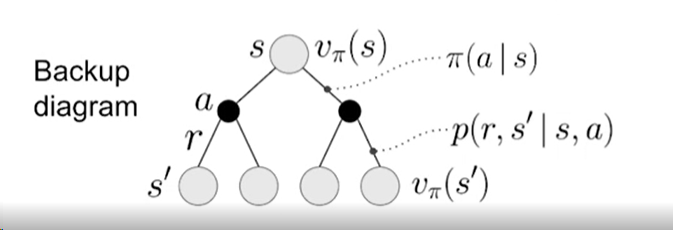
\includegraphics[width=1\linewidth]{../Image/screenshot002}
		\caption{Backup diagram for $v(s)$}
		\label{fig:screenshot002}
	\end{figure}
	
	$q(s)$ is calculated:
	
	$\begin{aligned} q_\pi(s, a) & =\sum_{r, s^{\prime}} p\left(r, s^{\prime} \mid s, a\right)\left[r+\gamma v_\pi\left(s^{\prime}\right)\right] \\ & =\sum_{r, s^{\prime}} p\left(r, s^{\prime} \mid s, a\right)\left[r+\gamma \sum_{a^{\prime}} \pi\left(a^{\prime} \mid s^{\prime}\right) q_\pi\left(s^{\prime}, a^{\prime}\right)\right]\end{aligned}$
	
	\begin{figure}
		\centering
		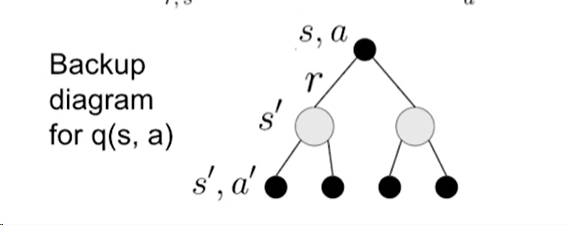
\includegraphics[width=1\linewidth]{../Image/screenshot003}
		\caption{Backup diagram for $q(s)$}
		\label{fig:screenshot003}
	\end{figure}
	
	\subsubsection{Bellman optimality equation}
	
	We could compare policies on the basis of $v(s)$
	
	$\pi \geq \pi^{\prime} \quad \Leftrightarrow \quad v_\pi(s) \geq v_{\pi^{\prime}}(s) \quad \forall s$
	
	$v_*(s)=\max _\pi v_\pi(s)$
	
	$q_*(s, a)=\max _\pi q_\pi(s, a)$
	
	\textbf{Notes: in any finite MDP there is always at least one deterministic optimal policy}
	
	$\begin{aligned} v_*(s) & =\max _a \sum_{r, s^{\prime}} p\left(r, s^{\prime} \mid s, a\right)\left[r+\gamma v_*\left(s^{\prime}\right)\right] \\ & =\max _a \mathbb{E}\left[R_t+\gamma v_*\left(S_{t+1}\right) \mid S_t=s, A_t=a\right]\end{aligned}$
	
	$\begin{aligned} q_*(s, a) & =\mathbb{E}\left[R_t+\gamma \max _{a^{\prime}} q_*\left(S_{t+1}, a^{\prime}\right) \mid S_t=s, A_t=a\right] \\ & =\sum_{r, s^{\prime}} p\left(r, s^{\prime} \mid s, a\right)\left[r+\gamma \max _{a^{\prime}} q_*\left(s^{\prime}, a^{\prime}\right)\right]\end{aligned}$
	
	   
	 \subsection{Generalized Policy Iteration}
	 
	 \begin{enumerate}
	 	\item Policy Evaluation 
	 	\item Policy Improvement
	 \end{enumerate}
 	
 	\subsubsection{Policy evaluation}
 	
 	Policy evaluation is also a called \textbf{prediction problem}.
 	
 	Predict value function for a particular policy
 	
 	Bellman expectation equation: 
 	
 	$$\begin{aligned} v_\pi(s) & =\sum_a \pi(a \mid s) \sum_{r, s^{\prime}} p\left(r, s^{\prime} \mid s, a\right)\left[r+\gamma v_\pi\left(s^{\prime}\right)\right] \\ & =\mathbb{E}_\pi\left[R_t+\gamma v_\pi\left(S_{t+1}\right) \mid S_t=s\right]\end{aligned}$$
 	
 	is basically a system of linear equation
 	
 	Algorithm:
 	
 	
 	\begin{figure}[H]
 		\centering
 		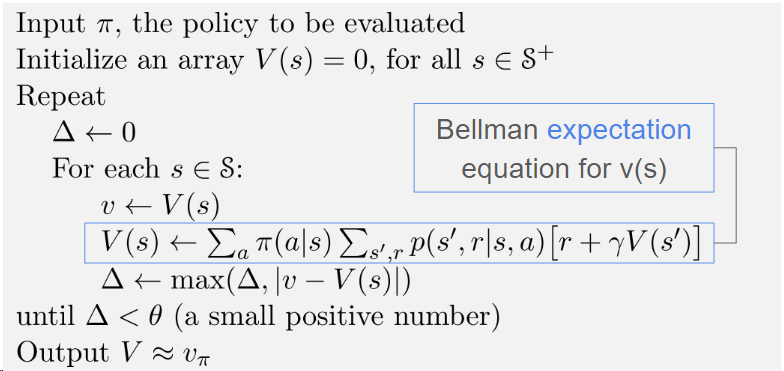
\includegraphics[width=1\linewidth]{../Image/screenshot004}
 		\caption{}
 		\label{fig:screenshot004}
 	\end{figure}

	\subsubsection{Policy improvement}
	
	Idea: once we know what $v(s)$ for a particular policy, we could improve it by acting greedily w.r.t v(s)!
	
	$$\pi^{\prime}(s) \leftarrow \underset{a}{\arg \max } \overbrace{\sum_{r, s^{\prime}} p\left(r, s^{\prime} \mid s, a\right)\left[r+\gamma v_\pi\left(s^{\prime}\right)\right]}^{q_\pi(s, a)}$$
	
	This procedure is guaranteed to produce a better policy. 
	 	
 	
	
	
	
	
	
\end{document}